\documentclass[12pt]{IEEEtran}
\usepackage{graphicx}
\usepackage[export]{adjustbox}
\usepackage{amsmath}
\usepackage{amssymb}
\usepackage{tabu}
\usepackage{multirow}
\usepackage{caption} 
\usepackage{float}
\usepackage{array}
\captionsetup{skip=1.1pt}

\begin{document}

\title{Concurrent and Distributed Computing}

\author{\IEEEauthorblockN{Enrico Aquilina}
\IEEEauthorblockA{\textit{Faculty of ICT}\\
\textit{University of Malta},\\
\textit{Msida, Malta}\\
\textit{enrico.aquilina.16@um.edu.mt}}}

\maketitle
\IEEEpeerreviewmaketitle


\section{Introduction}
This assignment describes my implementation of the n-body problem. It is divided into three main sections: running the program, techniques used for the implementation components and performance measurement design and analysis.

\section{Running the program}
In this section I will explain how to run my implementation. 

\subsection{Help menu}
The compiled version of the implementation has a small menu for help in case it is needed. This can be viewed by passing -h flag when running the compiled version of the program. Table 1 shows the help menu with a description explaining what each flag performs.

\begin{table}[ht]
\caption{Help functionality}
\centering 
\begin{tabular}{c c}
\hline
Flag & Flag description\\[0.5ex]
\hline
-h & help menu argument\\
-n & choose the number of particles(64, 1024, 4096, 16384) \\
-t & number of threads to use in the implementation\\
-o & specify whether the output logs are required\\
-r & specify which version to run: 0(seq), 1(omp), 2(mpi), 3(all)\\
[1ex]
\hline
\end{tabular}
\label{table:nonlin}
\end{table}

If the flags are not passed as arguments the implementation  sets its default parameters. The program sets the number of particles to 1024, the implementations to run to all and the number of threads to 12 and it sets the flag to not require output files to be printed.

\subsection{G++ compiler}
To compile the OpenMP implementation part I used the g++ compiler. I added the -fopenmp flag to include the GCC's OpenMP library in the terminal command. I also explicitly specified the version of C++ to use in the terminal by passing the -std flag. An example to compile the implementation for OpenMP would therefore be g++ -fopenmp -std=c++11 main.cpp. To execute the output, one would then do ./a.out.

\subsection{MPIC++ compiler}
I then proceeded to use the mpic++ compiler to compile the MPI relevant code. I used the -o flag to link to an output file and used the -fopenmp and -std flags as mentioned in the previous section. The final terminal command would be mpic++ -o mpi main.cpp -fopenmp -std=c++11. To run the compiled program in this case, one could issue mpirun -np 4 ./mpi -r 2 to run the MPI implementation only by using the r flag and using 4 processors specified by the -np flag.

\section{Discussion of thr techniques used for parallel decomposition}
In this section I will discuss how I parallelised the problem using OpenMP and MPI for the n-body problem.

\subsection{Naive shared memory implementation using OpenMP}
For the openMP implementation I used a few different directives. To improve the n-body problem performance I parallelised the outer loop which loops through all of the bodies. 
\medskip

To measure the time taken for OpenMP's implementation I used OpenMP's omp\_get\_wtime() to measure the wall clock time. I take the average out of three runs for each implementation and then compute the average to get a better estimate of the time taken.
\medskip

The outer loop of the naive n-body was parallelised using a few directives together. One of the directives which was amalgamated into the combined one was `num\_threads' to set the number of threads in my team of threads. The default number of threads was initially set to 12 based on the project specifications. For my personal machine, I specified 8 as the default because it seemed to return with better results.
\medskip

The following two directives which were used for the outer loop were OpenMP's `pragma omp parallel' and `pragma omp for'. These two could be combined to form `pragma omp parallel for' which would tell the compiler to initialise a team of threads and distribute the iterations of the loops among the spawned threads.
\medskip

For this directive I also specified the `private' directive which declares a list of variables private to a task. I declared the three vectors direction, distance and force to be private using this directive. For the computation of the force, I used the directive `pragma omp critical' to restrict execution of writing to the force vector such that only a single thread at a time  can edit the variable. 
\medskip

I also tried using locks by implementing `omp\_set\_lock', and I found that I obtained similar output results in both cases. However, I opted to use the `pragma omp critical' because on my personal machine it returned with slightly better performance time than `omp\_set\_lock'.
\medskip

For the acceleration computation and writing to the particles' velocities, I used `pragma omp critical', similar to the previous section. 
\medskip

I did not introduce any parallel constructs in the final implementation for computing the particles' positions because I don't think that is necessary and the computation done in the loop is relatively simple. Furthermore, I did do some runs with `pragma omp parallel for' directive but the time to compute was increased. Therefore no OpenMP directives were implemented in this section.

\subsection{Distributed implementation using MPI}
In this section I will discuss about the decomposition of my MPI implementation. This implementation starts off by initialising MPI and creating an MPI struct to hold the particle information. 
\medskip

The root process will first compute the size of the array holding the array of particles. It will then broadcast this count to the other processors for them to have a copy of the size of the bodies array. The MPI directive used here was MPI\_Bcast(\&bodiesSize, 1, MPI\_UNSIGNED, 0, MPI\_COMM\_WORLD). The bodiesSize is the reference to the size of the array, and 1 is referring that I'm sending one integer along.
\medskip

After computing and sending the size, the root process broadcasts the whole array to all the other processors. The directive used here is similar for passing the array count but \&bodies.front() is passed as the first argument as the address of the first element. The second argument, bodiesSize is passed as the second argument which is the count of particles which we are sending.
\medskip

The other processors will receive the bodies array count and a local copy of the bodies array for each processor. The directive used was MPI\_Bcast to receive the count. These processors will also receive the bodies array using MPI\_Bcast().
\medskip

The next directive which I used was MPI\_Wtime() to start measuring the time for the MPI implementation. The forces were then computed for each processor by calculating the count each processor has to process. In my case I assumed that the paricle count was equally divisible by the processors. After the computation of the forces, I placed a barrier using MPI\_Barrier(MPI\_COMM\_WORLD) to make sure all the processes have computed their share of particles' forces. 
\medskip

%At this stage, each process should have computed their chunk of particles.The implementation proceeds by each process computing the positions of all their particles arrays. The other computation for the particles' positions were calculated for each processor.
%\medskip

The next directive used was MPI\_Allgather() to send each processor's computed share of particles to every processor in order to update their bodies array. I implemented it this way to minimise network traffic instead of sending each processor's share of particles to the root and the root sending it to every processor to update their bodies array.
\medskip

I used MPI\_IN\_PLACE as the first argument to MPI\_Allgather to reference an intracommunicator. The second parameter which is the sendcount, referring to the data count being sent. I passed chunk in this case which was the particle count divided by the processor count. The third argument was the sendtype, where I used the MPI data type created earlier to hold my data about the particles. 
\medskip

The fourth argument which is the recvbuf, I used a pointer to the array of particles which contained the data received from each process. For the fifth argument, I specified chunk as the number of elements in the receive buffer. The sixth argument which is the recvtype, I specified the MPI\_ParticleType again.
\medskip

I conclude my MPI implementation by placing a barrier to make sure all processes have received all the particles' data from the other processes. Following this, I move the particles' positions at this stage. This is done for every processor to update their copy of the bodies array. This process is iterated for the number of steps defined.
\medskip

After the loop I recompute the time using MPI\_Wtime(). Then, I check whether it's the root process(rank 0) and output to the console the time taken for the MPI implementation.

\subsection{Shared and distributed implementation(OpenMP and MPI}
This implementation is a hybrid implementation of the shared memory and distributed implementation. This implementation starts similar to the distributed implementation by populating the bodies array and checking whether the current process is rank 0(root).
\medskip

The rank 0 process is responsible for sending the bodies data to all the processes to compute their respective chunks using MPI\_Bcast(). The processes then receive their copy of the bodies array and can continue processing.
\medskip

The counter is started at this point using MPI\_Wtime() and a for loop is initialised to loop one thousand times. In the method to compute the forces for each process I use OpenMP's `pragma omp parallel for' for the outer for loop which loops through the chunk of bodies which the processor needs to compute. 
\medskip

I used the OpenMP's private keyword for the variables direction, distance and force and passed the num\_threads directive the number of threads to be intialised for the force computation. Similar to the shared memory implementation I used `pragma omp critical' for computing the force. In the last part of the force computation method, I used `pragma omp critical' again to update the particle's velocity.

\section{Performance measurement design and analysis}
In this section, I will present the average time taken for the implementations to compute the problem for 16384 particles using the ALbert cluster.
 
\subsection{Sequential implementation}
The sequential implementation was the implementation which took the most time, resulting in an average of 40069 seconds.

\begin{table}[H]
\centering
\captionsetup{justification=centering}
\renewcommand{\arraystretch}{1.3}
\begin{tabular}{|c|c|}
\hline
   & Time(seconds)\\
\hline
  Run 1 & 40007.9 \\
\hline
  Run 2 & 40053.6 \\
\hline
  Run 3 & 40145.8 \\
\hline
  Average & \textbf{40069.1} \\
\hline
\end{tabular}
\end{table}	

\subsection{Naive shared memory implementation using OpenMP}
The OpenMP implementation using 12 processing elements was the second fastest implementation with an average time of 7078 seconds.
\begin{table}[H]
\centering
\captionsetup{justification=centering}
\renewcommand{\arraystretch}{1.3}
\begin{tabular}{|c|c|}
\hline
   & Time(seconds)\\
\hline
  Run 1 & 7050.8\\
\hline
  Run 2 & 7023.9\\
\hline
  Run 3 & 7161.7\\
\hline
  Average & \textbf{7078.6}\\
\hline
\end{tabular}
\end{table}	

\subsection{Distributed implementation using MPI}
The MPI distributed implementation using 4 cores was the third fastest implementation with an average time of 12077 seconds.
\begin{table}[H]
\centering
\captionsetup{justification=centering}
\renewcommand{\arraystretch}{1.3}
\begin{tabular}{|c|c|}
\hline
   & Time(seconds)\\
\hline
  Run 1 & 12072.8\\
\hline
  Run 2 & 12150.9\\
\hline
  Run 3 & 12009.6\\
\hline
  Average & \textbf{12077.8}\\
\hline
\end{tabular}
\end{table}	

\subsection{Hybrid implementation using shared and distributed memory}
This implementation was the fastest of all the implementations which used 4 nodes and 12 cores with an average time taken of 5127 seconds.
\begin{table}[H]
\centering
\captionsetup{justification=centering}
\renewcommand{\arraystretch}{1.3}
\begin{tabular}{|c|c|}
\hline
   & Time(seconds)\\
\hline
  Run 1 & 5007.9 \\
\hline
  Run 2 & 5084.6\\
\hline
  Run 3 &  5290.8\\
\hline
  Average & \textbf{5127.7}\\
\hline
\end{tabular}
\end{table}	

\section{Analysis and speed-up comparison of the different implementations}
This sections shows a plot showing the difference observed by using various numbers of processing elements from my implementations. The x-axis represents the number of processing elements used taking values of 1, 4, 12 and 48 processing elements representing the sequential, distributed, shared memory and hybrid implementations respectively. The y-axis represents the time taken for each implementation running the 16384 particle input file which is represented in seconds.
\medskip

The longest implementation was the sequential one which took 40069 seconds, followed by the distributed implementation using MPI getting slightly better results with an average of 12077 seconds, followed by the OpenMP implementation with an average of 7078 seconds and finally the hybrid implementation with the best results of 5127 seconds. The results are plotted in the figure below. 

\begin{figure}[H]
	\centering
	\begin{center}
	\centering
		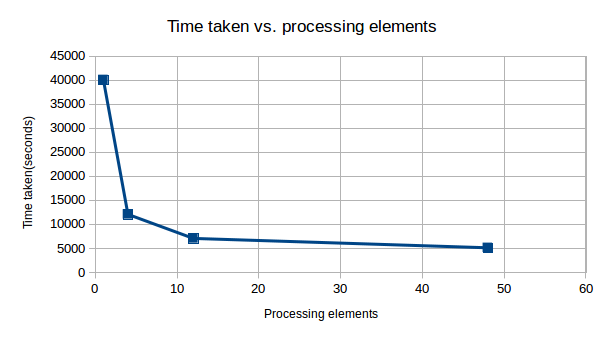
\includegraphics{speedups2}	
	\end{center}
\end{figure}

The output files for the 64, 1024 and 4096 particles can be found in the Dropbox link(https://www.dropbox.com/sh/b2vghhcesyxq38q/
AADFw2mxDYHGJxL1MAu28CZAa?dl=0).
\end{document}


